\documentclass{report}
\usepackage[utf8]{inputenc}
\usepackage{amsmath, amsfonts, amsthm}
\usepackage{graphicx}
\usepackage{lipsum}
\usepackage{multicol}
\usepackage{geometry}
\usepackage{tcolorbox}
\usepackage[skip=20pt, indent=0pt]{parskip}

% \setlength{\hoffset}{-1in}
% \setlength{\voffset}{-1in}
% \setlength{\marginparwidth}{1.5in}
% \setlength{\oddsidemargin}{0in}


\newtheorem{theorem}{Theorem}[section]
\newtheorem{corollary}{Corollary}[theorem]

\newcommand{\R}{\mathbb{R}}
\newcommand{\cv}[2]{\begin{bmatrix}
        #1 \\
        #2 \\
    \end{bmatrix}}

\title{Hello World!}
\author{Alec Gideon}
\date{\today}

\begin{document}
\maketitle
\section*{Introduction}
Let's begin with a formula $e^{i\pi} +1=0$.

\begin{itemize}
    \item But we can also do

          $$
              \lim_{n \to \infty} \left(1+\frac{1}{n}\right)^n = \lim_{n \to \infty} \frac{n}{\sqrt[n]{n!}}
          $$

    \item We can do another:

          $$
              e=\sum_{n=0}^{\infty} \frac{1}{n!}
          $$

    \item We can also use conitnued fractions

          $$
              e = 2 + \frac{1}{1 + \frac{1}{2 + \frac{2}{3 + \frac{3}{4+\ddots}}}}
          $$
\end{itemize}

\section*{More Formulas}

$$ \int_{a}^{b}f(x)dx$$

%$$ \iiint f(x,y,z) dxdydz$$

$$ \vec{v} = <v_1,v_2,v_3>$$

$$\vec{v}\cdot \vec{w} $$

$$
    \begin{bmatrix}
        1 & 2 & 3 \\
        4 & 5 & 6 \\
    \end{bmatrix}
$$

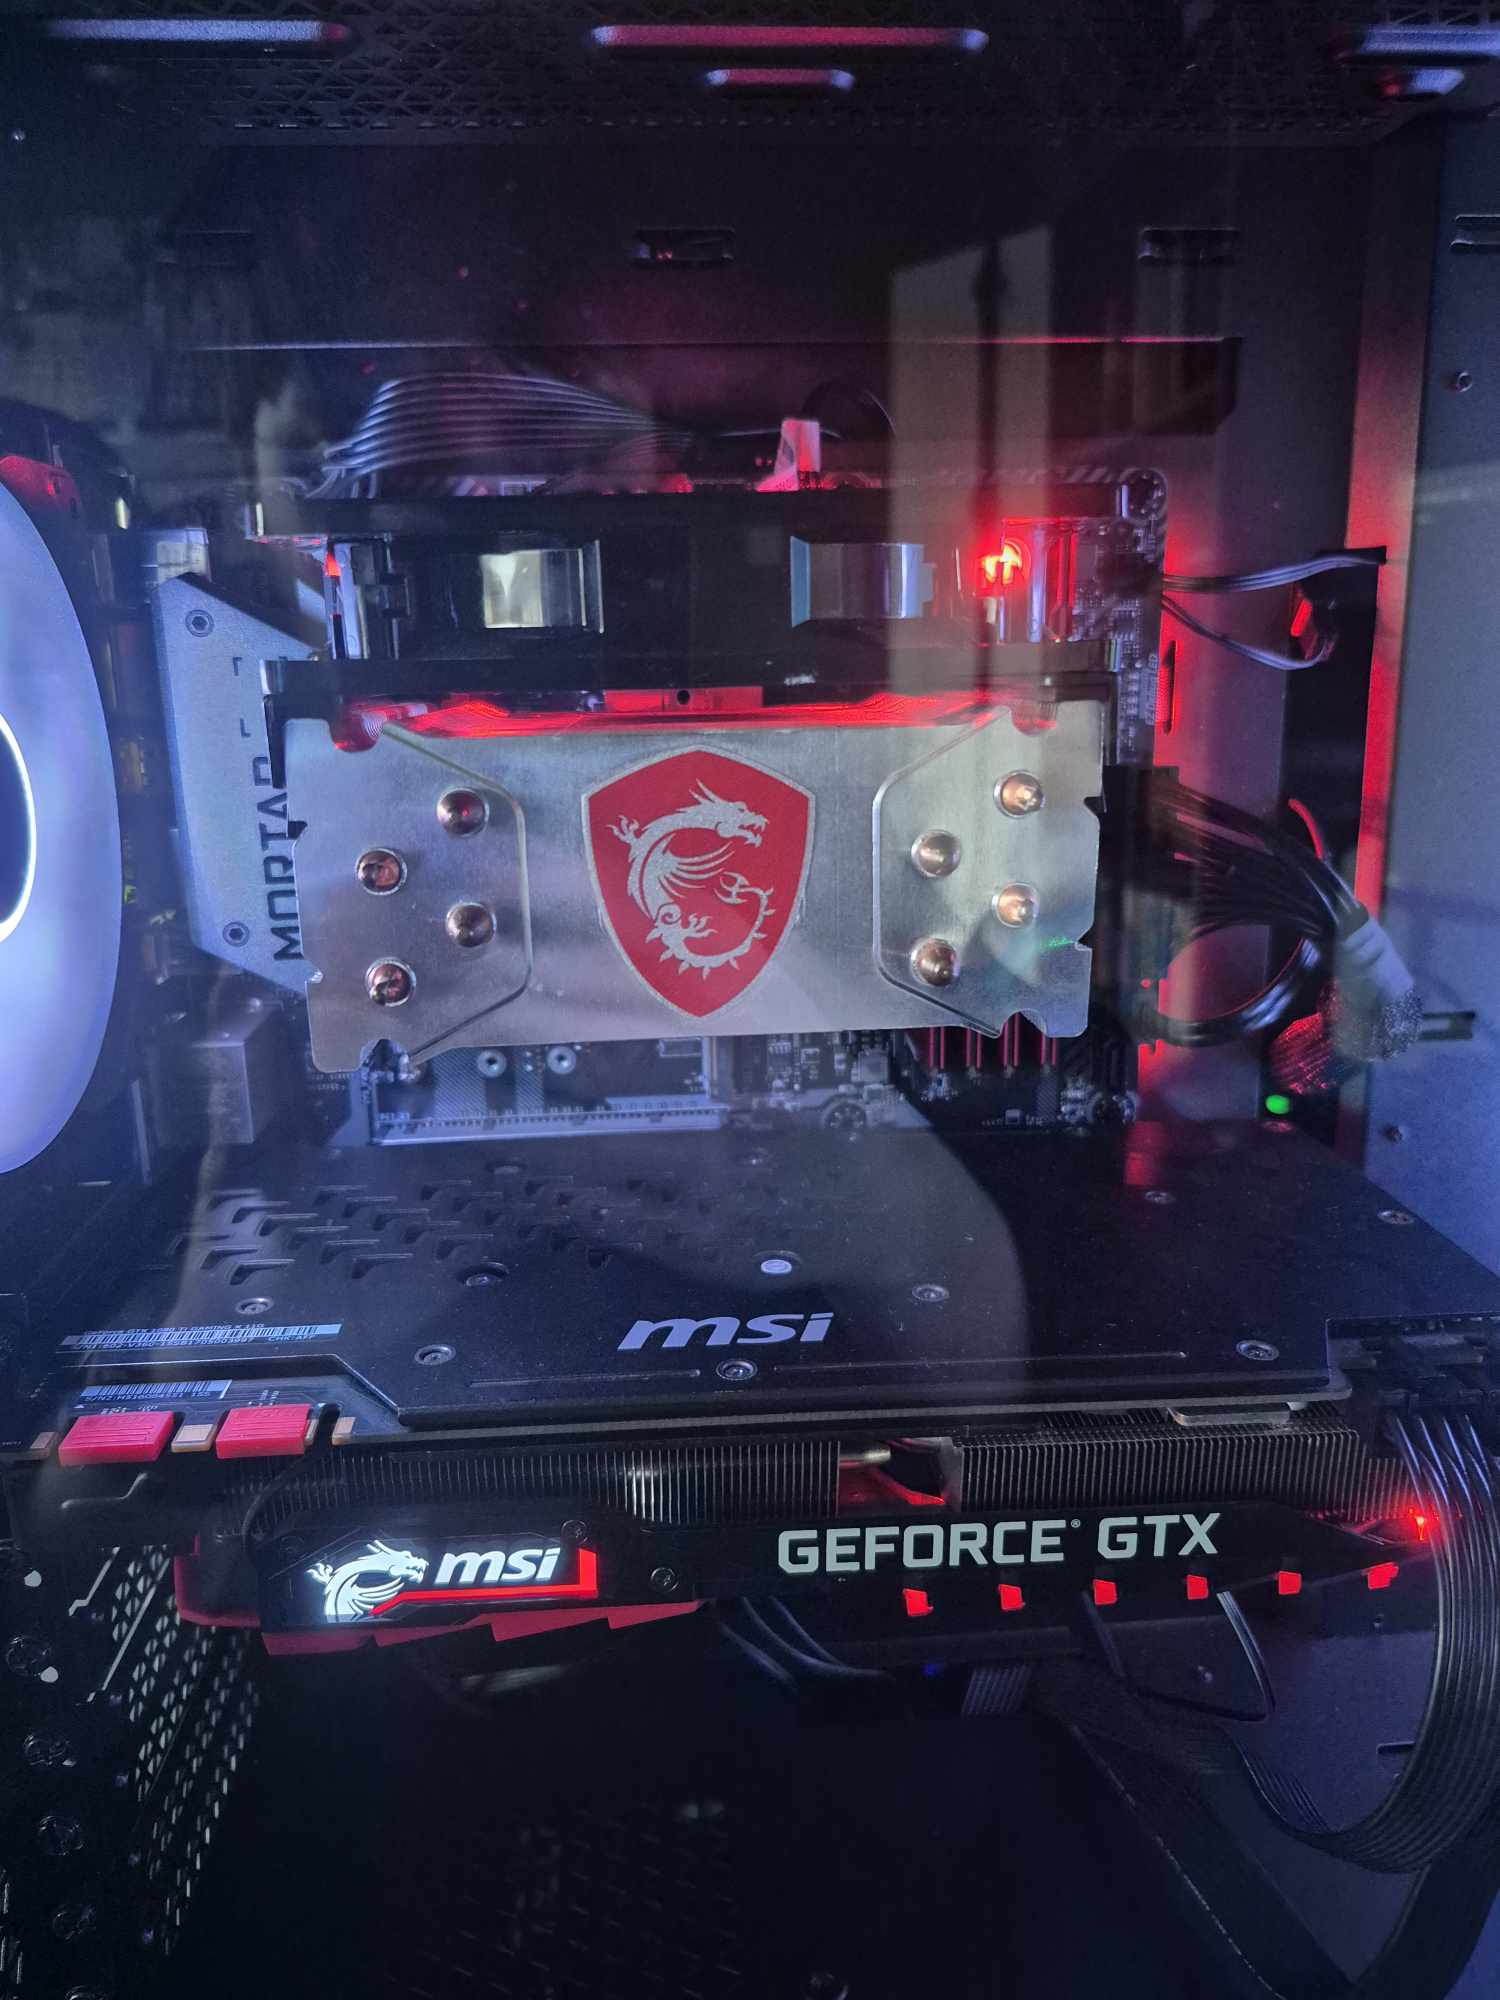
\includegraphics[scale=0.1]{cooler.jpg}

\section{Definitions of $e$}
\begin{enumerate}
    \item As a \textbf{limit}:
          \begin{equation}
              \begin{split}
                  e & = \lim_{n \to \infty} \left(1 + \frac{1}{n}\right)^n \\
                    & =\lim_{t \to 0}(1 + t)^{\frac{1}{t}}
              \end{split}
          \end{equation}
    \item As a \textit{sum}:
          \[e = \sum_{n=0}^{\infty}\frac{1}{n!}\]
          \begin{multline}
              e^x \approx 1 + x + \frac{x^2}{2} + \frac{x^3}{3!} + \frac{x^4}{4!}
              + \frac{x^5}{5!} + \frac{x^6}{6!} + \frac{x^7}{7!} \\ + \frac{x^8}{8!} + \frac{x^9}{9!} + \frac{x^{10}}{10!} + \frac{x^{11}}{11!} + \frac{x^{12}}{12!} + \frac{x^{13}}{13!}
          \end{multline}
    \item As a \underline{continued fraction}:
          \[e =2 + \frac{1}{1 + \frac{1}{2 + \frac{2}{3 + \frac{3}{4 + \frac{4}{5 + \ddots}}}}}\]
\end{enumerate}

\newpage

\section{More Tricks}

\begin{table}
    \caption{A nifty table!}
    \label{niftyTable}
    \begin{center}
        \begin{tabular}{|c|r|}
            \hline
            1 & 2         \\
            \hline
            3 & 400000000 \\
            \hline
        \end{tabular}
    \end{center}
\end{table}

I like table \ref{niftyTable}

\begin{figure}
    \centering
    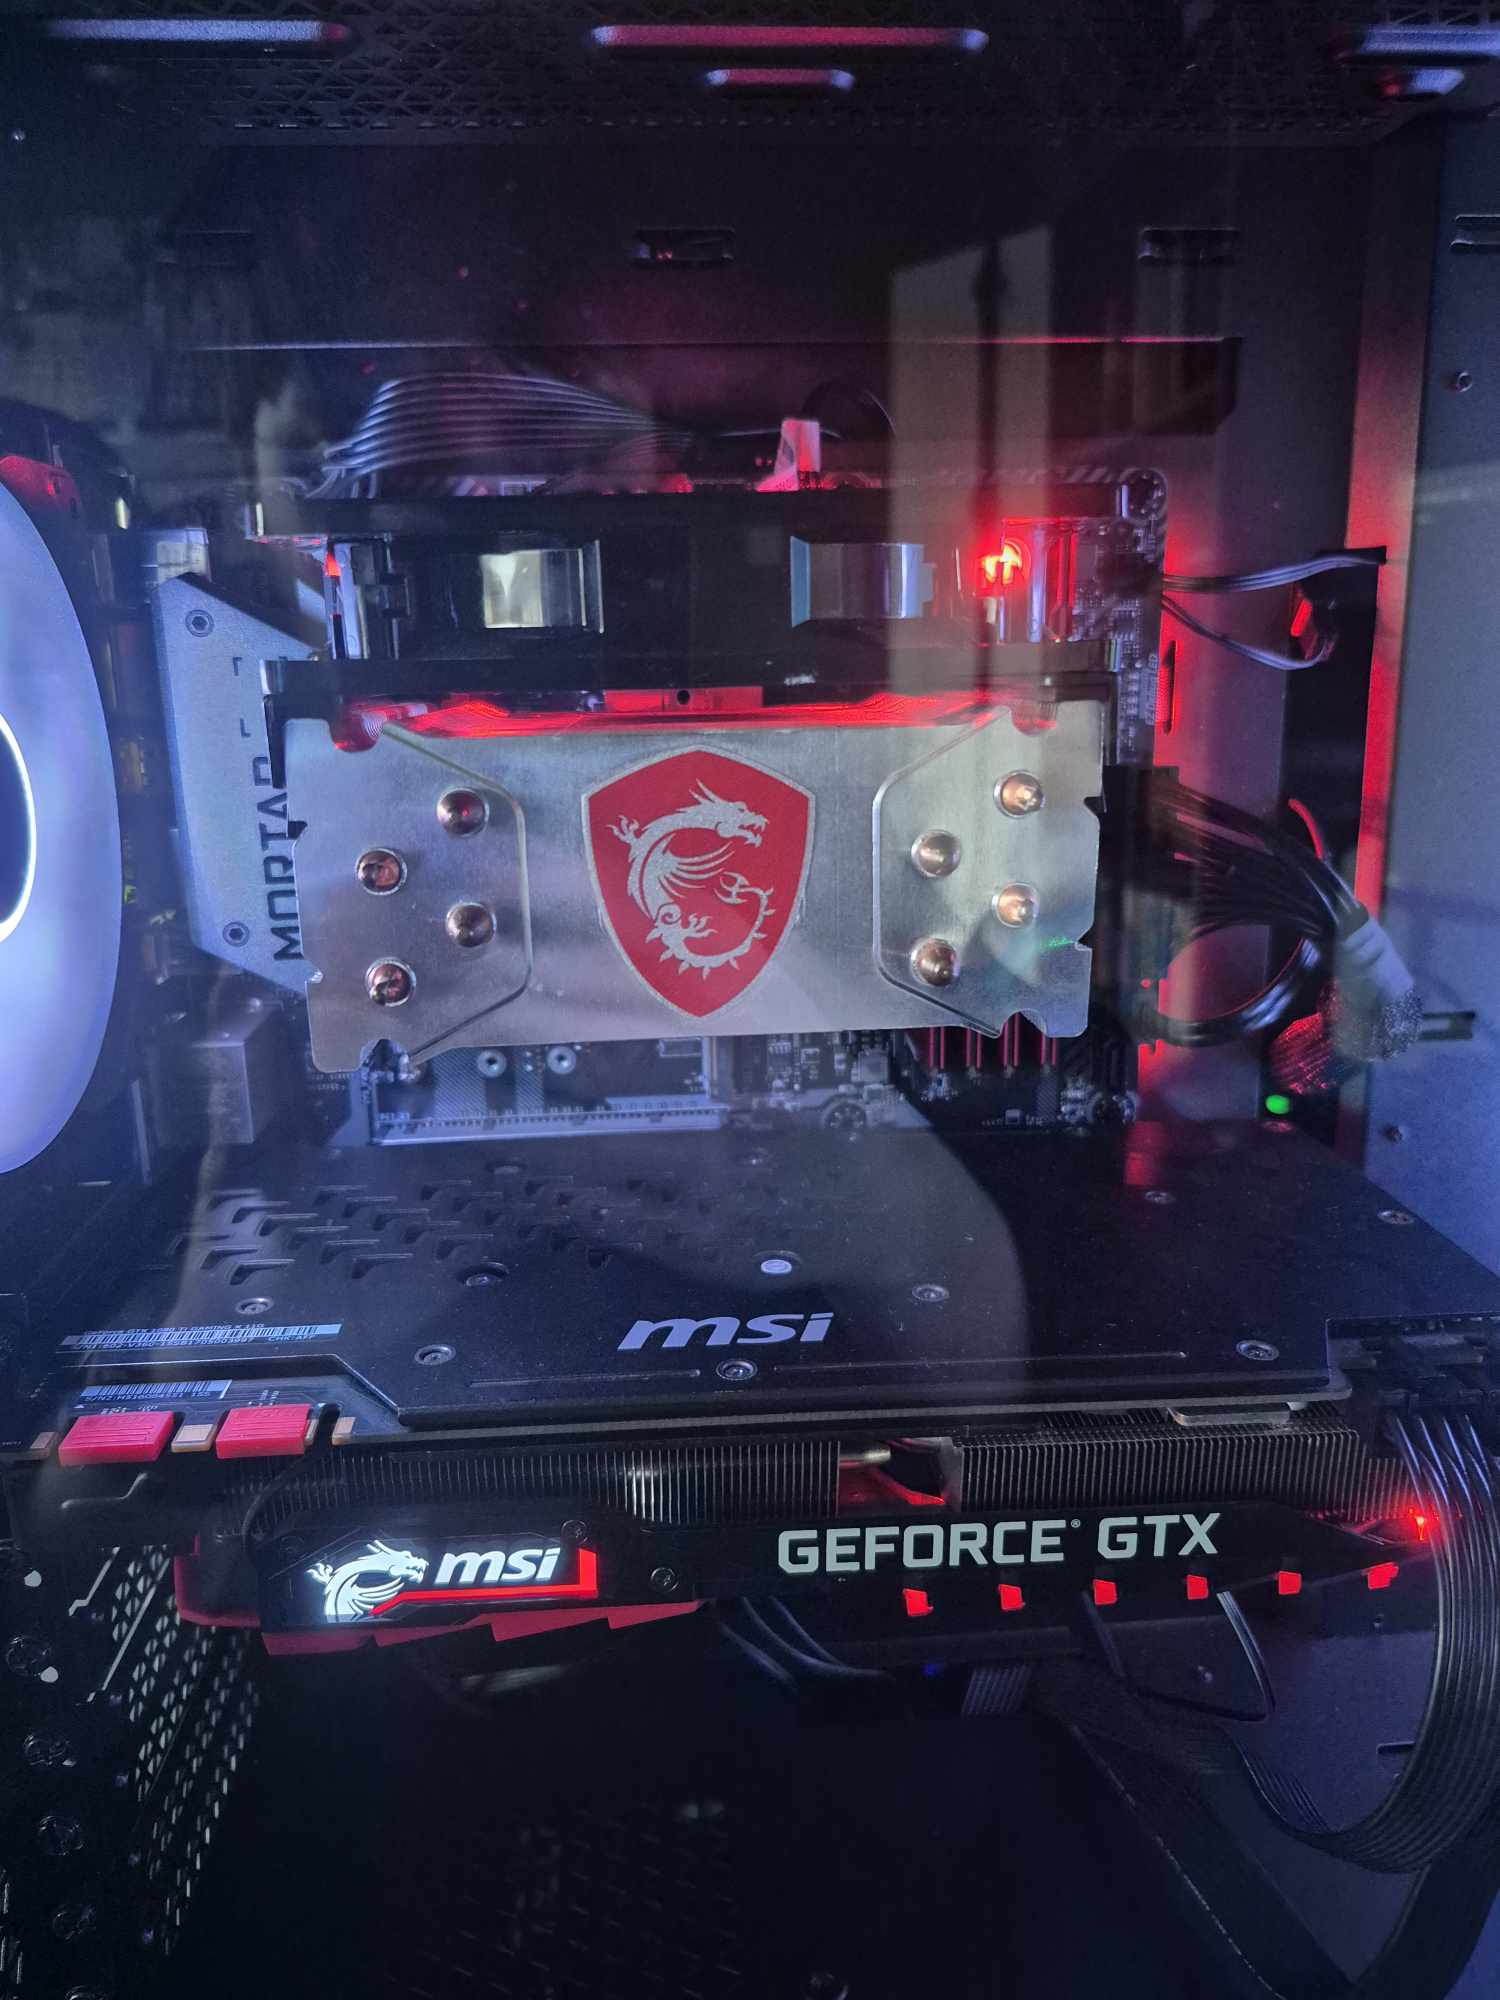
\includegraphics[width=\textwidth]{cooler.jpg}
    \caption{I did it}
    \label{cooler}
\end{figure}

I am so proud of figure \ref{cooler}

\newpage

\begin{theorem}[YouTube Theorem]
    You should like and subscribe!
\end{theorem}
\begin{proof}
    Left to the interested subscriber
\end{proof}

\begin{theorem}
    You should like and subscribe and ring the bell!
\end{theorem}

\begin{corollary}
    And check out Overleaf as well
\end{corollary}

The real numbers $\R$

I could do \[\begin{bmatrix}
        a \\
        b \\
    \end{bmatrix}\]

I could do $\cv{1}{2}$

\subsection{Columns}
\begin{itemize}
    \item twocolumn
    \item multicols
    \item Minipage
\end{itemize}

\lipsum[1-5]

\newpage
\begin{multicols*}{2}[This stuff in square brackets is an optional preamble to the following columns. You can think of it as a header]
    \lipsum[1-5]
\end{multicols*}

\begin{minipage}{0.6\textwidth}
    \lipsum[1]
    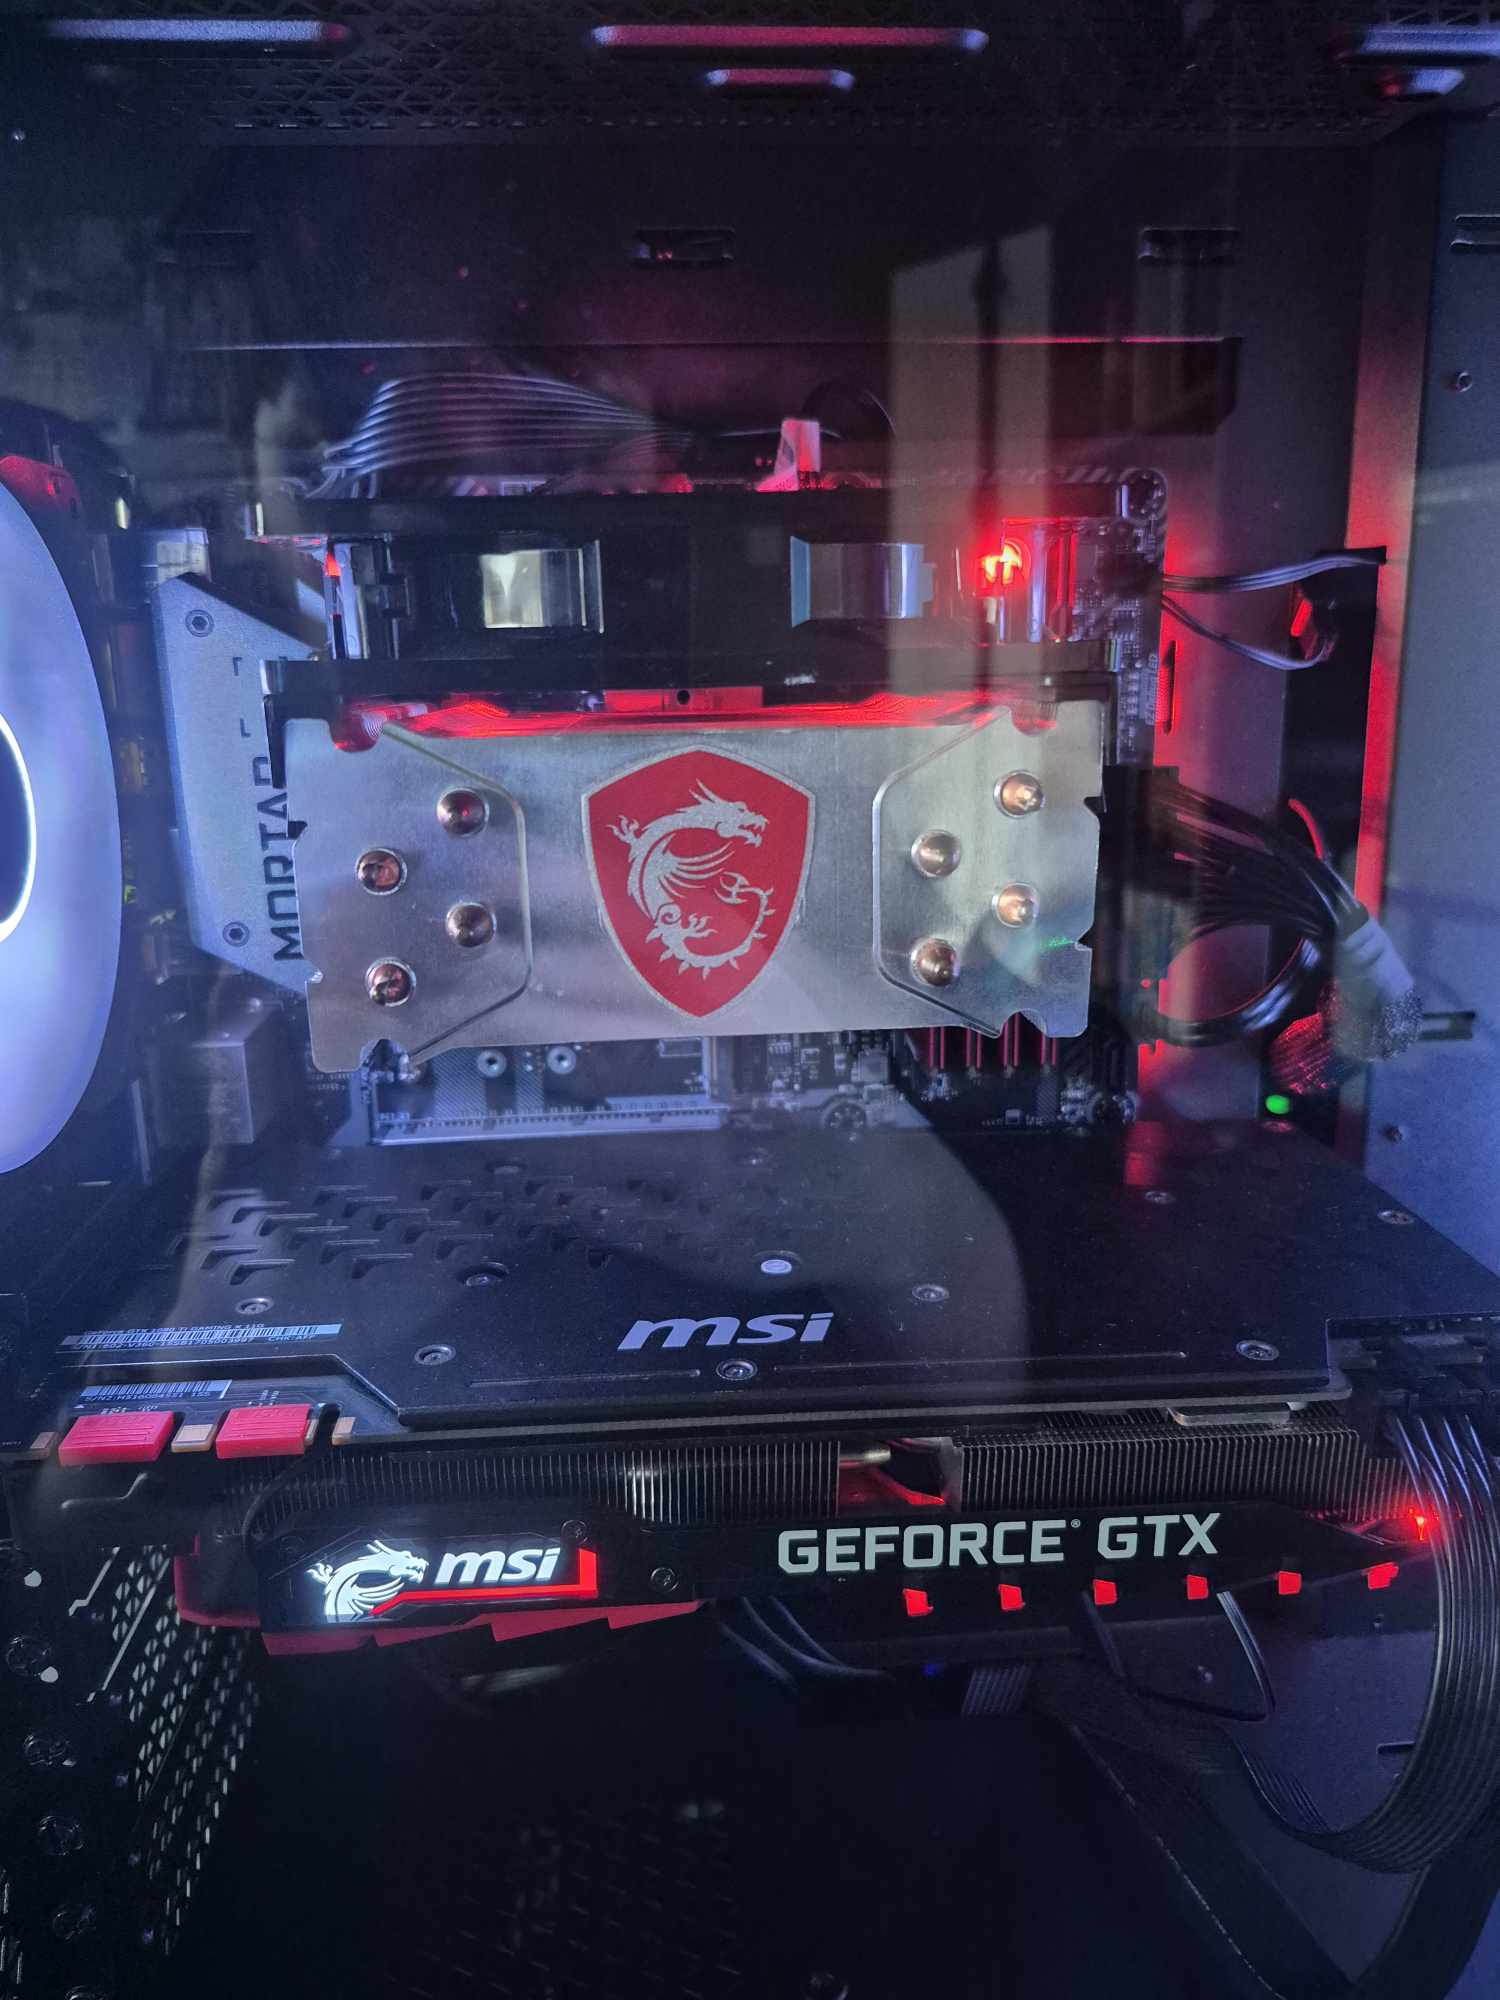
\includegraphics[width=\linewidth]{cooler.jpg}
\end{minipage}
\hspace{10pt}
\begin{minipage}{0.3\textwidth}
    \lipsum[1]
    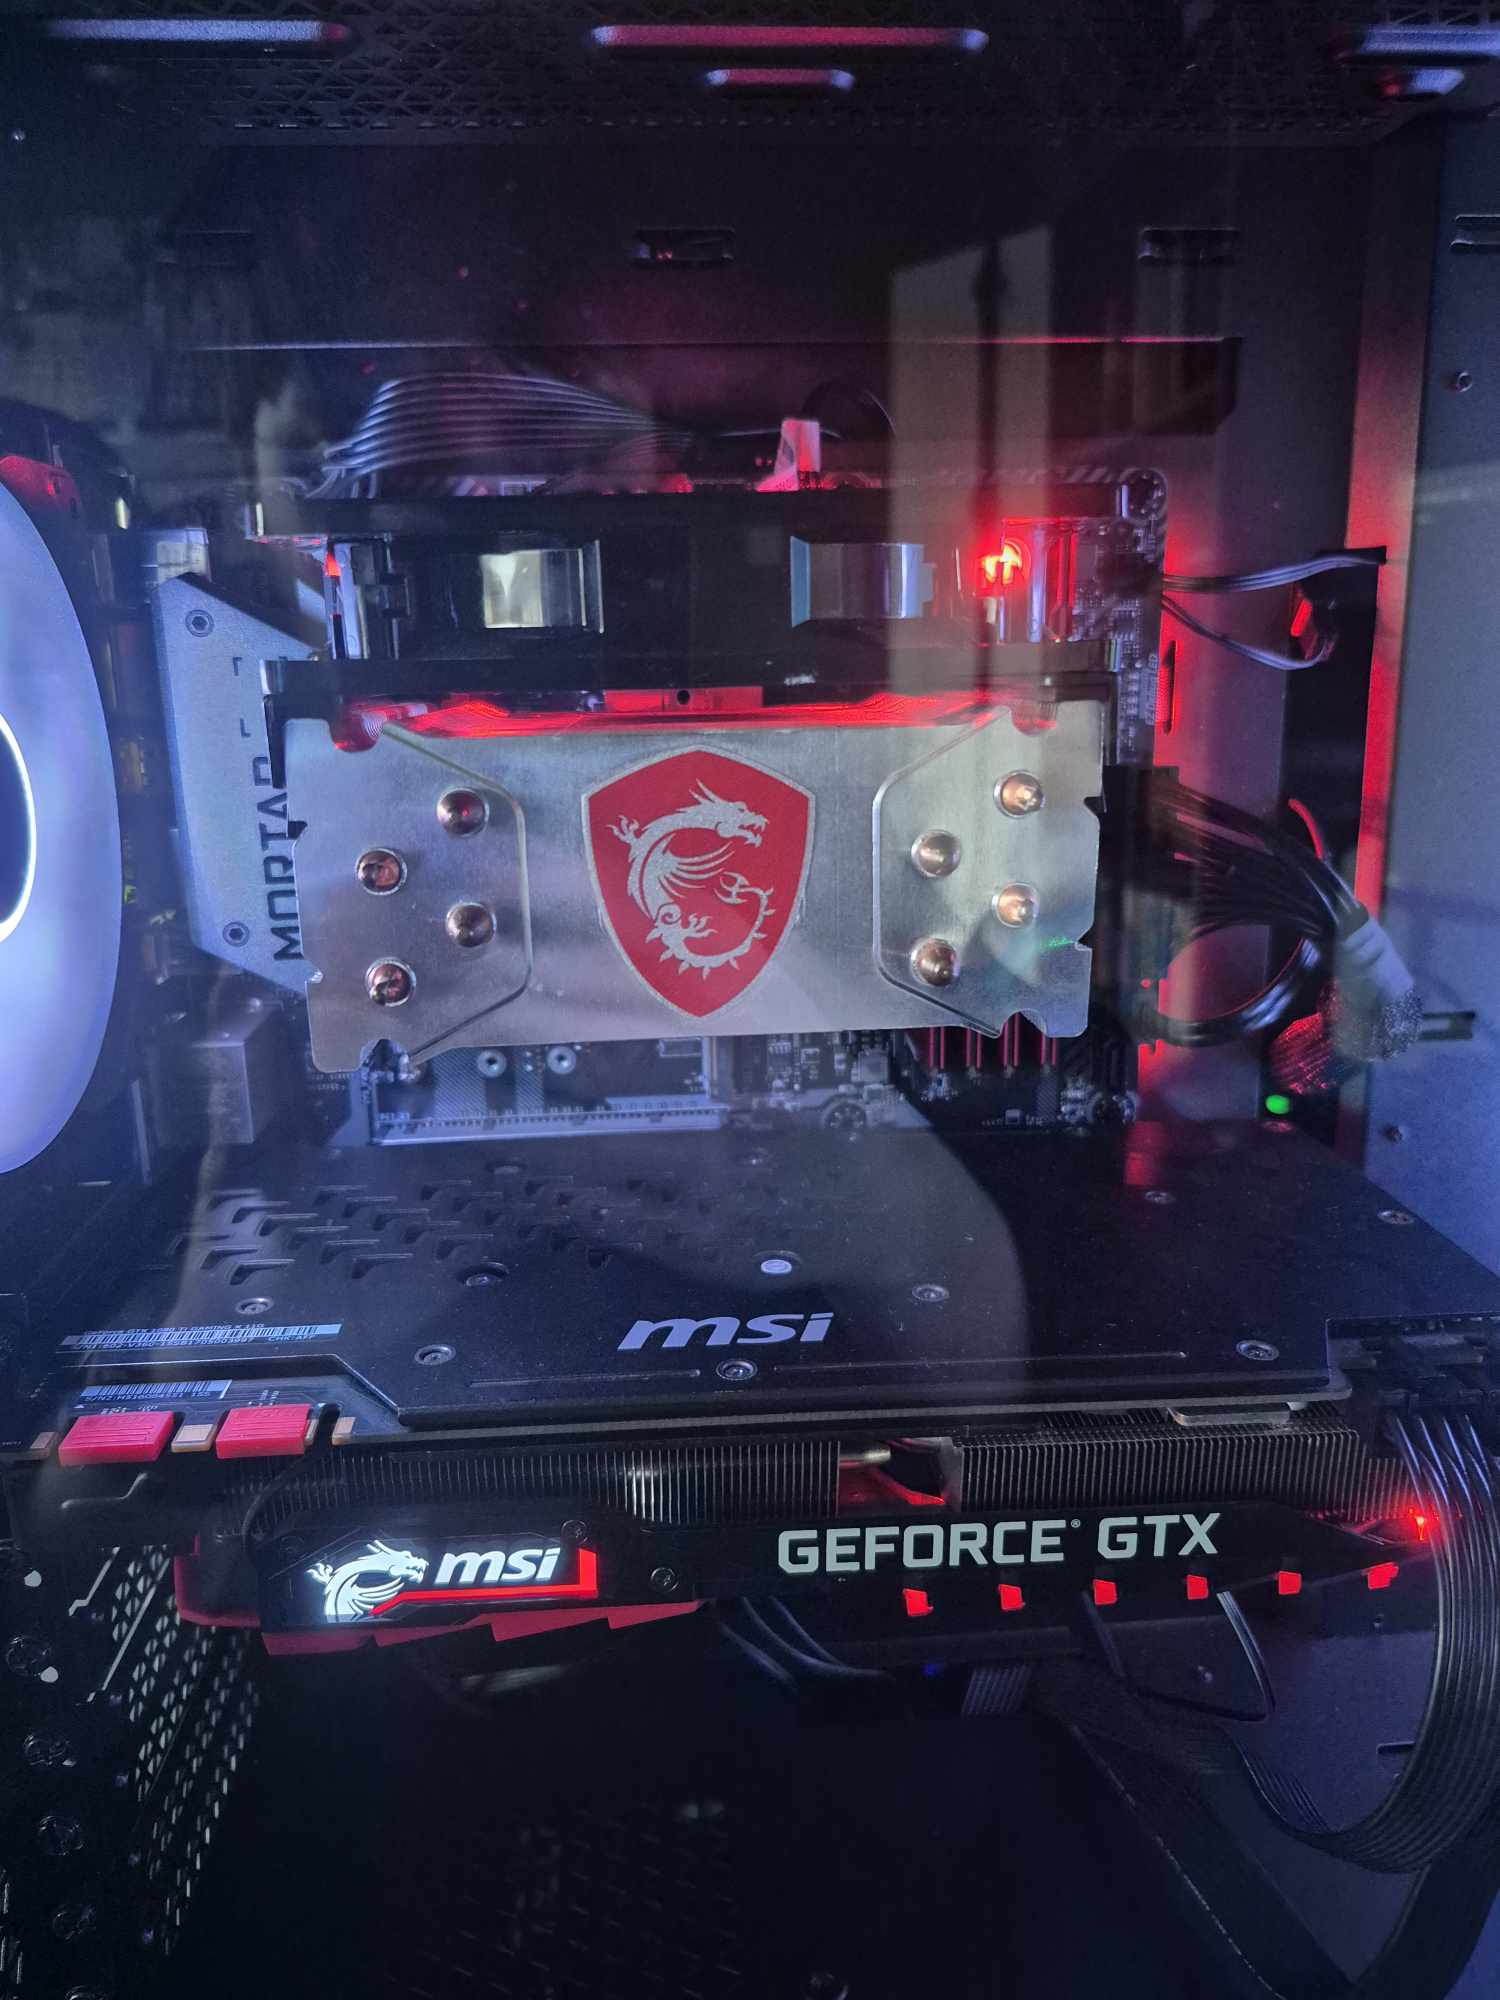
\includegraphics[width=\linewidth]{cooler.jpg}
\end{minipage}

\subsection{Margins}
\begin{itemize}
    \item Margins
    \item Margin Notes
\end{itemize}

Lorem ipsum dolor sit amet, consectetuer adipiscing elit.
Ut purus elit, vestibulum ut, placerat ac, adipiscing vitae,
felis. Curabitur dictum gravida mauris. Nam arcu libero,
nonummy eget, consectetuer id, vulputate a, magna. Do-
nec vehicula augue eu neque \marginpar{This is a margin note}. Pellentesque habitant morbi
tristique senectus et netus et malesuada fames ac turpis
egestas. Mauris ut leo. Cras viverra metus rhoncus sem.
Nulla et lectus vestibulum urna fringilla ultrices. Phasellus
eu tellus sit amet tortor gravida placerat. Integer sapien
est, iaculis in, pretium quis, viverra ac, nunc. Praesent eget
sem vel leo ultrices bibendum. Aenean faucibus. Morbi
dolor nulla, malesuada eu, pulvinar at, mollis ac, nulla.
Curabitur auctor semper nulla. Donec varius orci eget ri-
sus. Duis nibh mi, congue eu, accumsan eleifend, sagittis
quis, diam. Duis eget orci sit amet orci dignissim rutrum

\subsection{Whitespace}
\begin{itemize}
    \item \verb|\hfill| vs \verb|\hspace| vs \verb|\ | vs \verb|\quad|
    \item \verb|\vfill| vs \verb|\vspace| vs \verb|\bigskip|
\end{itemize}

\[y'' + y' + y = 0, y(0) = 0, y'(0) = 1\]
\[y'' + y' + y = 0,\  y(0) = 0,\  y'(0) = 1\]
\[y'' + y' + y = 0,\quad  y(0) = 0,\qquad  y'(0) = 1\]
\[y'' + y' + y = 0,\hspace{1in}  y(0) = 0,\hspace{1in}  y'(0) = 1\]

This is some text \hfill This is some other stuff

\vfill

This is some more text \newpage

\subsection{Linebreaks and Paragraph Spacing}
\begin{itemize}
    \item \verb|\\| vs double return
    \item \verb|\parskip|
    \item No indent
\end{itemize}

\noindent This is a Paragraph.

This is a second Paragraph. \\ This is a new line

\subsection{Annotating Equations}

\begin{itemize}
    \item Underbaces
    \item witharrow package
    \item colorbox
\end{itemize}

\end{document}
